\documentclass[11pt]{book}

\usepackage[width=7.0in, height=9.0in, top=1.0in, papersize={8.5in,11in}]{geometry}
\usepackage[pdftex]{graphicx}
%\usepackage{datetime}
\usepackage{anyfontsize}
\usepackage{hyperref}
\usepackage{t1enc}
\usepackage{verbatim}
\usepackage{algorithm}
\usepackage{algorithmic}
\usepackage{framed}
\usepackage{pdfpages}
\usepackage{listings}
\lstset{language=C}

\lstset{language=python,frame=ltrb,framesep=5pt,basicstyle=\normalsize,
 keywordstyle=\ttfamily\color{DarkRed},
%morecomment=[n][\textbf]{In\ [}{]\:},
%morecomment=[n][\textbf]{Out\ [}{]\:},
morecomment=[s][\color{blue}]{In\ [}{]\:},
morecomment=[s][\color{red}]{Out[}{]\:},
identifierstyle=\ttfamily\color{DarkBlue}\bfseries,
commentstyle=\color{DarkGreen},
stringstyle=\ttfamily,
showstringspaces=false,tabsize = 3}


\lstdefinelanguage{shell} {
commentstyle = \color{black},
keywordstyle = \color{black},
stringstyle = \color{black},
identifierstyle = \color{black},
morecomment=[s][\color{blue}]{In\ [}{]\:},
morecomment=[s][\color{red}]{Out[}{]\:},
 }

\pagestyle{empty}
\title{Sprint \#2 Prototype}
\date{11/04/15}
\author{Team Expeditus}
\usepackage{helvet}
\renewcommand{\familydefault}{\sfdefault}
\begin{document}
\maketitle
\noindent The purpose of this document is to review the demonstrable work products from Sprint 2. These work products are:
\begin{itemize}
\item Visual Homography for Autonomous Landing
\item Simulation
\item Purchasing UAV Parts 
\end{itemize}

\section*{Visual Homography for Autonomous Landing}
\large{\textbf{Introduction}}\\
\normalsize
\noindent The purpose of this report is to give a brief overview of the current status of the existing code from the 2014-2015 landing pad team's repository. Fortunately, it appears that much of the code is reusable. If not in full, parts of the code can be pulled from the repository to get the ball rolling. In the report, we'll go through where to find the existing code in the repository, and what it's currently capable of.\\
\vspace{2mm}\\
\noindent\large{\textbf{Location in Repository and Building Source}}\\
\normalsize
\noindent The code being discussed throughout is in the GitHub repository \href{https://github.com/SDSMT-CSC464-F15/landingpad/tree/master/2014-2015/led}{here}. To run this code on your local machine (assuming you have opencv installed as well as the latest compilers) navigate to the above directory, and type 'cmake .'. Then, run make. Once you've done this, you can run the code with './tracker'. Assuming you're on your school laptop, it'll automatically access the front-facing camera, and you'll see a happy little picture of your smiling face! I'm assuming that you're happy, since you've just succeeded in getting the software to run. As this runs, you may notice that it draws some circles and coordinates on the video feed. This overlay is meant to point out the positions of the RGB blobs in the frame. We've taken the large printout of the AR tag and RGB blobs that the team used last semester, and tested the code with it. Fortunately, it works! You can see the results of this in the image below.\\
	
	\begin{figure}[h]
		\centering
		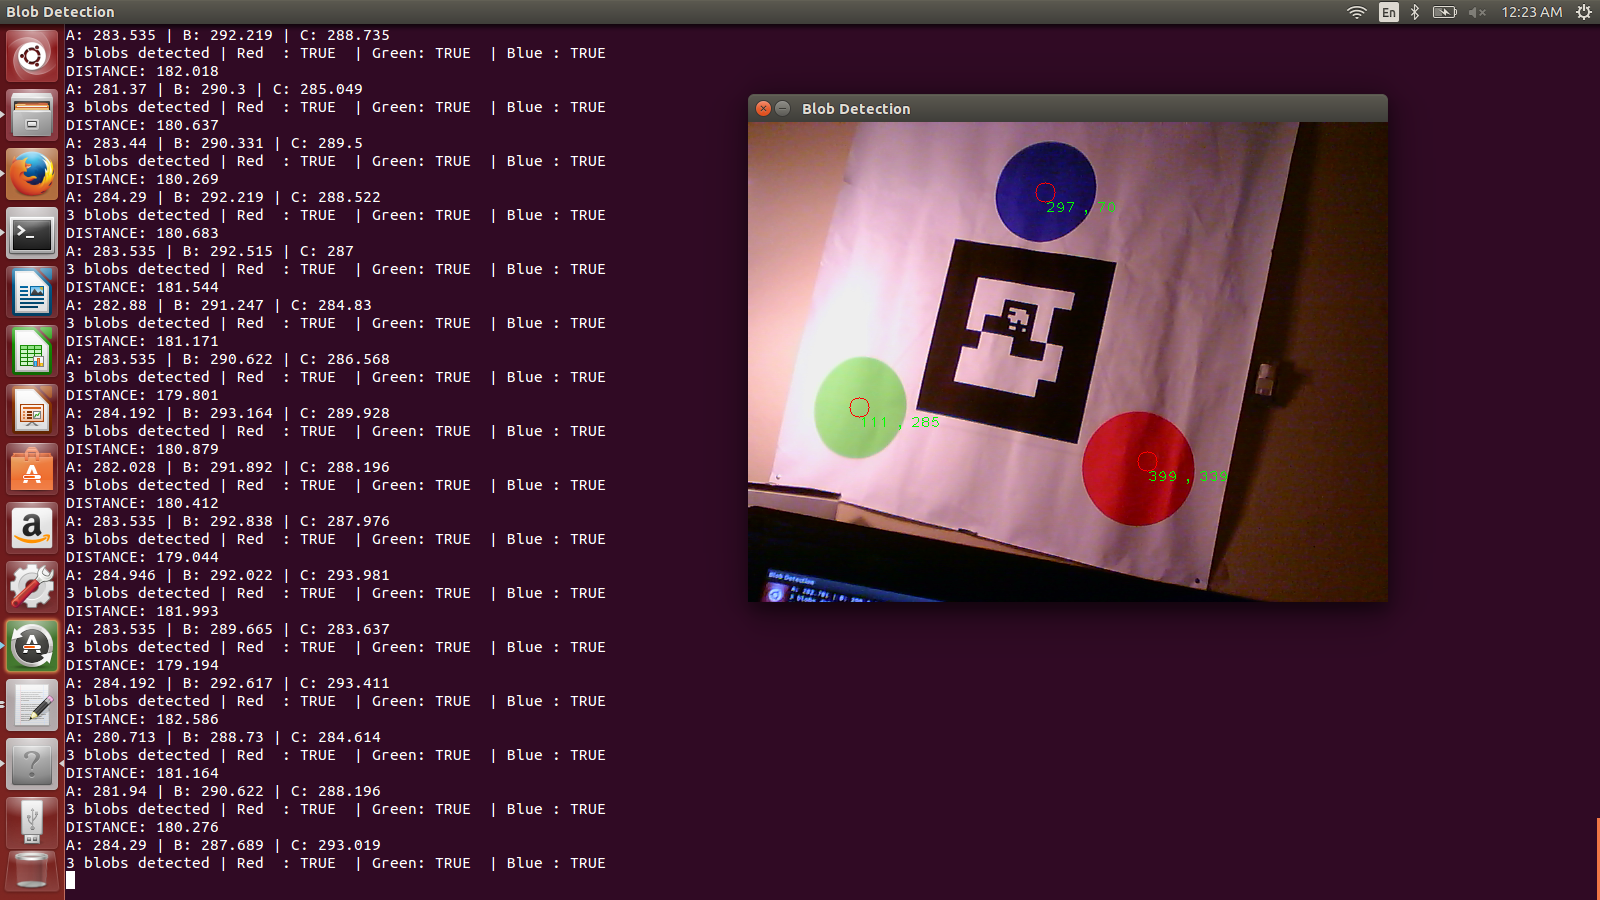
\includegraphics[width=0.8\textwidth]{coolpic.png}
		\caption{Blobs Detected}
	\end{figure}

\vspace{2mm}
\noindent\large{\textbf{Next Steps}}\\	
\normalsize	
\noindent Since the existing code outputs a correct distance in centimeters, the next step will to be able to detect the angle of the image. This will allow us to determine orientation. Since we have working code, we should just be able to clean it up, and copy it over into a new branch of our current repository. From there, we will begin to develop orientation detection!

\section*{Simulation}
\large{\textbf{Introduction}}\\
\normalsize
\noindent To test our landing algorithms in simulation, it would be very useful to have something that approximates the Pixhawk flight controller to communicate with for the purpose of supplying instructions to the controller, as well as receiving flight data. The PX4 development team have provided both Software-In-The-Loop and Hardware-In-The-Loop simulation meta-packages for use in ROS.\\
\vspace{2mm}\\
\large{\textbf{Build Instructions}}\\
\normalsize
\noindent This will require Linux 14.04, ROS Distro Indigo or Jade, and the installation of a few repositories. These are detailed well in the setup document provided by the group \href{https://pixhawk.org/dev/ros/sitl#px4_ros_sitl_setup}{here}. More roughly, after installation of the Ubuntu 14.04 and ROS Jade, other dependencies will need to be installed. After which, a number of repositories from GitHub will need to be cloned into the ROS workspace src directory. These repos include PX4/Firmware, PX4/rotors\_ simulator, PX4/mav\_ comm, ethz-asl/glog\_ catkin, and catkin/catkin\_ simple. \\
\noindent However, there were some issues found in following the instructions. For a successful build, it is easier to run each line of code from the provided bash scripts. Often, updates would fail, and the remainder of the script would fail to execute. Additionally, the \textbf{catkin\_ make} command did not build the meta-package correctly, as detailed in the instructions. It would repeatedly fail in finding the correct path to necessary files for the build. Rather, \textbf{catkin build} will build the meta-package properly and the simulation will run with the assistance of an XBox controller (PS controllers will not work). \href{https://www.youtube.com/watch?v=qfFF9-0k4KA}{Here} is a demonstration of the SITL meta-package created by the PX4 Autopilot Project.\\ 

\vspace{2mm}
\noindent\large{\textbf{Next Steps}}\\	
\normalsize	
\noindent We will next begin building our commands to the simulated Pixhawk through the use of the MavLink API, implemented as MavROS for use in the ROS environment. We will also test the HITL loop to ensure that our commands are being received by the actual hardware. 


\section*{Purchasing UAV Parts}
\large{\textbf{Introduction}}\\
\normalsize
\noindent  Over the course of Sprint 2, the team met with our advisor and faculty for purpose of receiving funding to create a new UAV platform for this project. The team also met with members of the UAV team to receive assistance and guidance in purchasing hardware that would be compatible with UAV team hardware. In the event of a component not functioning, our team would be able to utilize a component from the UAV team. After building a parts list for a hexrotor, we received approval from faculty for our purchase. Following is a list of the parts list with links to the pages containing information regarding the component.\\
\vspace{4mm}\\
\large{\textbf{Parts List}}\\
\normalsize
\vspace{2mm}\\
\begin{tabular}{l | c| r | r}

\textbf{Item} & \textbf{\#} & \textbf{Unit Cost} & \textbf{Unit Total}\\
\hline
\href{http://hobbyking.com/hobbyking/store/__23790__Turnigy_Talon_Hexcopter_V1_0_Carbon_Fiber_Frame_625mm.html}{Frame} & 1 & \$79.99 & \$79.99  \\
\href{http://www.hobbypartz.com/05m-11-mc3525-850kv-14p.html}{Motors} & 8 & \$23.99 & \$191.92 \\
\href{http://www.hobbypartz.com/07e04-proton-30a.html}{ESCs} & 8 & \$17.78 & \$142.24 \\
\href{http://store.3drobotics.com/products/3dr-pixhawk}{Pixhawk} & 1 & \$199.99 & \$199.99 \\
\href{https://store.3drobotics.com/products/hexacopter-power-distribution-board-1}{Power Distribution} & 1 & \$19.99 & \$19.99 \\
\href{https://store.3drobotics.com/products/gps-mast}{GPS Mast} & 2 & \$10.00 & \$20.00 \\
\href{http://store.3drobotics.com/products/3dr-gps-ublox-with-compass}{GPS} & 2 & \$89.99 & \$179.98 \\
\href{https://store.3drobotics.com/products/apm-power-module-with-xt60-connectors}{Power Module} & 1 & \$24.99 & \$24.99 \\
\href{http://ameridroid.com/products/odroid-xu4}{ODroid XU4} & 1 & \$75.95 & \$75.95 \\
\href{http://hobbyking.com/hobbyking/store/__39773__Carbon_Fiber_Propeller_10x4_7_Black_CW_CCW_4pcs_.html}{Props} & 3 & \$7.55 & \$22.65 \\
\hline
\textbf{TOTAL} & & & \$957.70 \\
\end{tabular}

\vspace{6mm}
\noindent\large{\textbf{Next Steps}}\\	
\normalsize	
\noindent After receiving the parts, the UAV will be assembled. After assembly, the team will be able to test flight control, which will provide feedback concerning a correctly assembled and functioning UAV. Afterwards, we will be able to test the autonomy in the flight controller, which will provide information regarding accuracy in waypoint navigation. 


\end{document}